\documentclass[onecolumn,12pt]{IEEEtran}

\usepackage[left=1in,right=1in,bottom=0.95in,nohead,nofoot]{geometry}
\usepackage{graphicx}

\begin{document}
\title{Informe Laboratorio 1}
\author{Redes de Datos}
%\vspace{3mm}

\begin{figure}[h]
\includegraphics[width=0.50\textwidth]{logo_udp.png}
\label{fig:mesh1}
\\
\\
\\
\\
\\
\maketitle
\end{figure}
\begin{center}
Integrantes:\\
\hfill \\
Gonzalo Felipe\\
Andres Hernandez\\
Franco Centeno\\
\hfill \\
\hfill \\
\hfill \\
\hfill \\
\\ \hfill \\
Profesor:\\
Jose Perez\\ \hfill \\
Ayudante:\\
Alexis Inzunza\\
\end{center}

\newpage
\title{Indice}
\author{ }
\maketitle
\hrule
\tableofcontents


\newpage
\section{IDENTIFICACION DE ELEMENTOS DE RED}
\hfill \\

\textbf{Identificar equipos conectados a la red:}\\ \hfill \\
Equipos HP EliteDesk 800 G1 SFF\\ \hfill \\
Intel(R) Core(TM) i7-4470 CPU @ 3.40GHz 3.39GHz\\

\textbf{Identificar el o los switch de la topolog�a:} \\ \hfill \\
Switch Catalyst 2960 Series\\

\textbf{Identificar hardware de red en general considerando la marca y modelo de los mismos:} \\ \hfill \\
Intel(R) Ethernet Connection I217-LM\\

\textbf{Identificar el tipo de cableado utilizado:} \\ \hfill \\ 
Cable Fast link USQ high technology data twist UTP 4PR 24AWG category 5E UL\\

\textbf{Identificar patch panel:} \\ \hfill \\ 
Patch HD Series\\

\newpage
\section{INFORMACION DE LOS DISPOSITIVOS}
\hfill \\

\textbf{Dispositivo 1:}\\ \hfill \\
IPv4: 172.16.32.107\\
Mask: 255.255.255.0\\
MAC: 40:A8:F0:4E:E8:E3\\

\textbf{Dispositivo 2:}\\ \hfill \\
IPv4: 172.16.30.66\\
Mask: 255.255.255.0\\
MAC: 40:A8:F0:52:CC:38\\

\textbf{Dispositivo 3:}\\ \hfill \\
IPv4: 172.16.30.77\\
Mask: 255.255.255.0\\
MAC: 40:A8:F0:5E:4F:28\\

\textbf{Dispositivo 4:}\\ \hfill \\
IPv4: 172.16.30.76\\
Mask: 255.255.255.0\\
MAC: 40:A8:F0:46:AB:51\\

\newpage
\section{DIAGRAMA DE LA TOPOLOGIA}
\begin{figure}[!h]
\caption{Diagrama de la topologia}
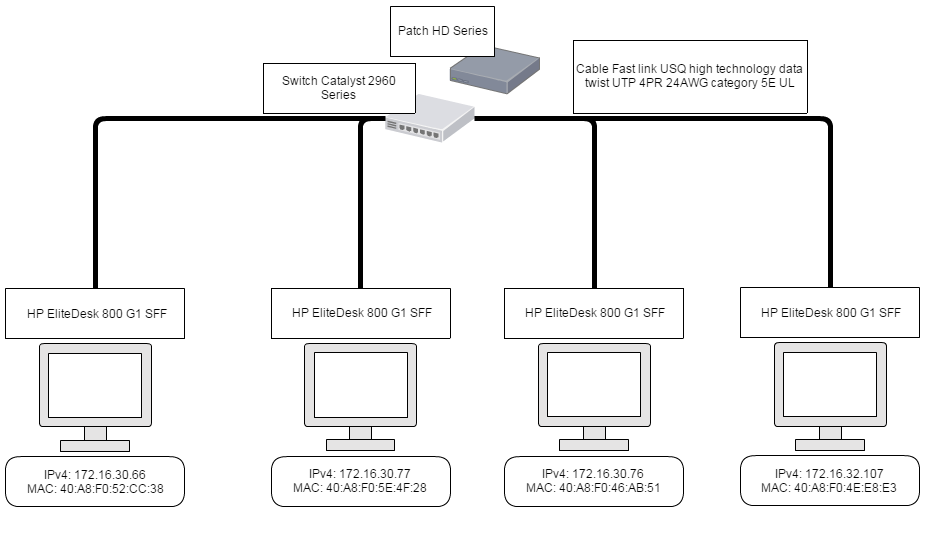
\includegraphics[width=1.1\textwidth]{Topologia.png}
\end{figure}

\newpage
\section{CONCLUSIONES}
\hfill \\

Asi como hemos podido reconocer la red del laboratorio, las conexiones desde un switch hasta los dispositivos, reconocer el cableado y el tipo de topologia usada, tambien nos hemos dado cuenta de los aspectos basicos, como los equipos y tipos de elementos necesarios para establecer cualquier red en cualquier parte.
\section{IMAGENES}
\begin{figure}[h!]
\centering
\caption{Patch y Switch}
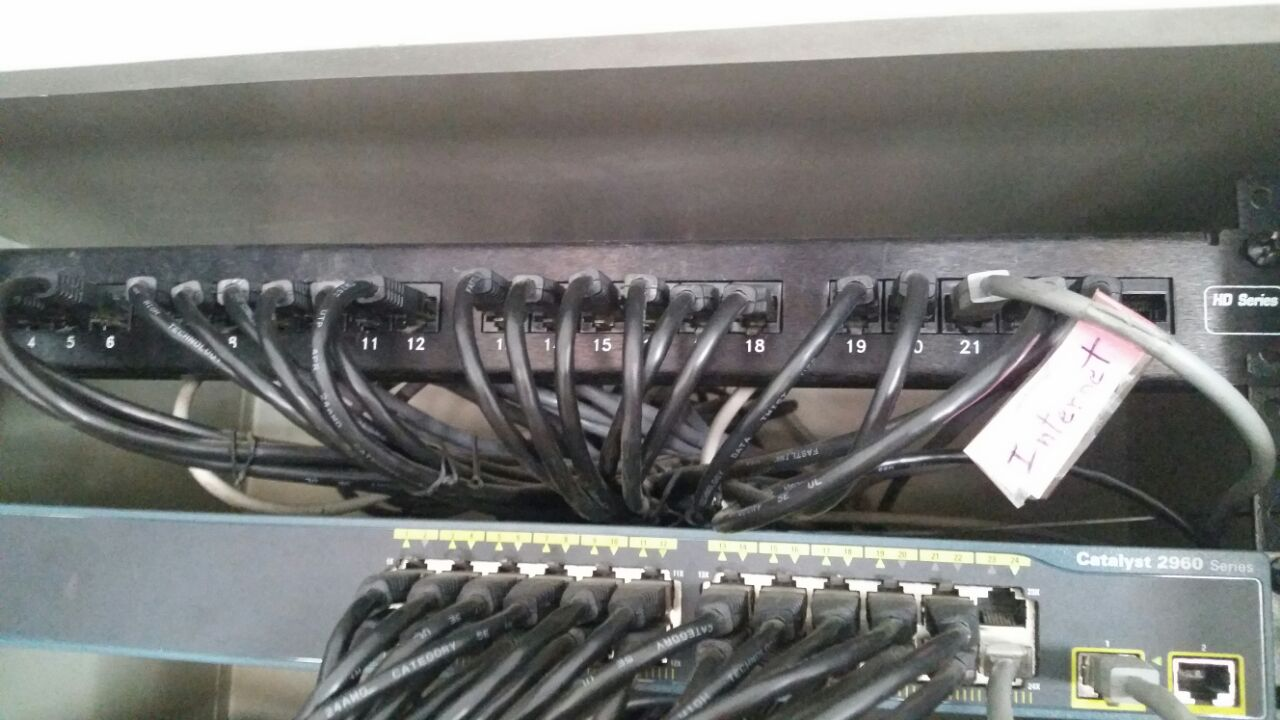
\includegraphics[width=0.50\textwidth]{PatchSwitch.jpg}
\caption{Cable UTP}
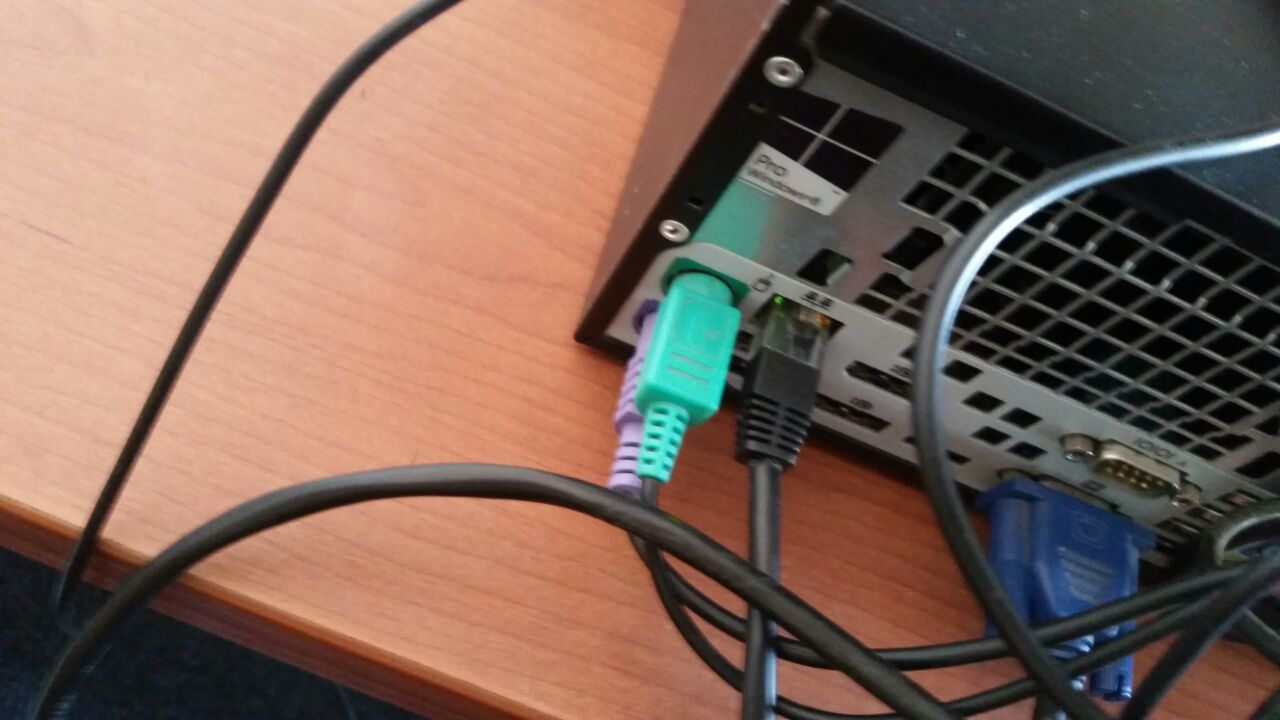
\includegraphics[width=0.50\textwidth]{UTP.jpg}
\end{figure}

\end{document} 